\documentclass{ctexart}
\usepackage{multicol}
\usepackage{amsmath, amsfonts, amssymb}
\usepackage{tikz, tkz-graph}
\usepackage{pgffor}
\usepackage{pifont}
\usepackage{nicematrix}
\usepackage{subfigure}
\usepackage{geometry}
\special{dvipdfmx:config z 0} % delete this when release

\usetikzlibrary{positioning}

\geometry{a4paper,scale=0.8}

\title{集合论与图论~作业15-17}
\author{庄嘉毅}
\date{November 2022}

\def\QED{\hfill $\square$}
\def\st{\textrm{s.t.}\,}
\def\pair#1{\left\langle #1 \right\rangle}
\def\conj{\mathrel{\wedge}}
\def\disj{\mathrel{\vee}}
\def\equ{\mathrel{\Leftrightarrow}}
\def\restr{\mathbin{\upharpoonright}}
\def\ple{\mathrel{\preccurlyeq}}
\DeclareMathOperator{\dom}{dom}
\DeclareMathOperator{\ran}{ran}
\DeclareMathOperator{\fld}{fld}
\DeclareMathOperator{\card}{card}
\DeclareMathOperator{\e}{e}

\everymath{\displaystyle}
% \linespread{2}

\begin{document}

\maketitle

\section*{习题八}

\paragraph*{4} 必要性: 若 $v_0$ 是可以任意行遍的, 假设 $G-v_0$ 中有圈,
那么存在一条从$v_0$开始且包含这个圈的欧拉回路, 把这个圈去掉, 由$v_0$是任意行遍的,
剩余的回路应该仍是欧拉回路, 矛盾. 因此 $G-v_0$ 中没有圈.

充分性: 若 $G-v_0$ 中没有圈, 由$G$是欧拉图,
知$G$是若干个边不重的圈的并, 并且所有圈都经过 $v_0$.
那么从$v_0$开始的任意行遍中, 每次回到$v_0$时, 都走完了 $G$ 的一个圈,
此时可以归纳地将这个圈从 $G$ 中删掉, 剩余的图仍满足条件,
由归纳法可知, 最终 $G$ 中的所有圈都被删掉, 此时行遍的路径是欧拉回路. \QED

\paragraph*{7}

\subparagraph*{(1)} 考虑图中 16,17,18,19,20 五个顶点, 将它们删去后,
图的连通分支数变为$7>5$, 因此原图不是哈密顿图.

\begin{figure}[ht]
    \centering
    \subfigure[]{
        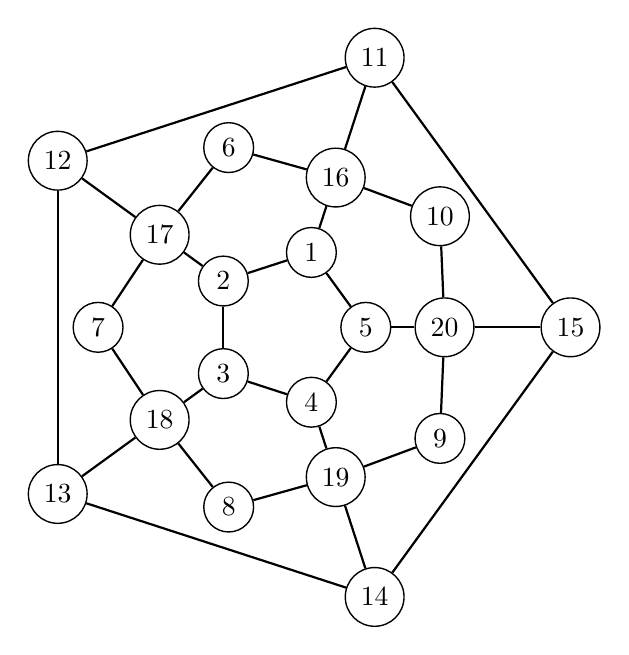
\begin{tikzpicture}
            \GraphInit[vstyle=Normal]
            \foreach \t in {1,...,5}{%
                    \Vertex[a=0+72*\t,d=1cm]{\t}
                }
            \foreach \t in {6,...,10}{%
                    \Vertex[a=36+72*\t,d=2.4cm]{\t}
                }
            \foreach \t in {11,...,15}{%
                    \Vertex[a=0+72*\t,d=3.6cm]{\t}
                }
            \foreach \t in {16,...,20}{%
                    \Vertex[a=0+72*\t,d=2cm]{\t}
                }
            \Edges(1,2,3,4,5,1)
            \Edges(6,17,7,18,8,19,9,20,10,16,6)
            \Edges(11,12,13,14,15,11)
            \Edges(1,16,11)
            \Edges(2,17,12)
            \Edges(3,18,13)
            \Edges(4,19,14)
            \Edges(5,20,15)
        \end{tikzpicture}}
    \quad
    \subfigure[]{
        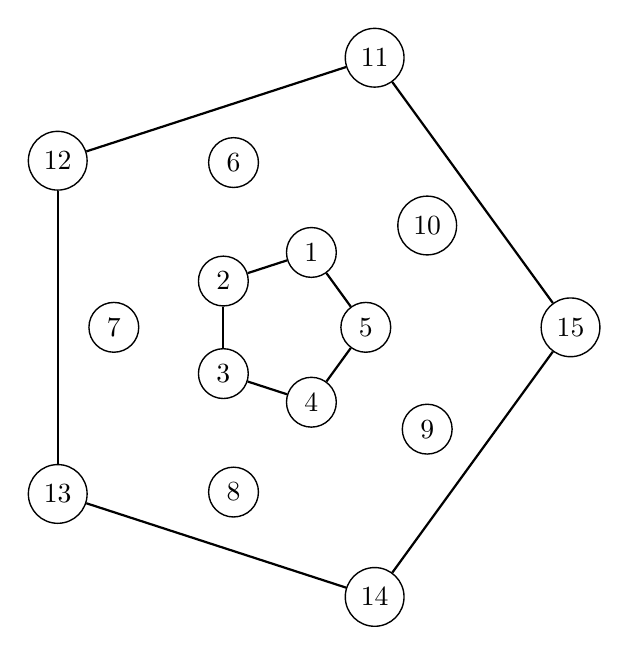
\begin{tikzpicture}
            \GraphInit[vstyle=Normal]
            \foreach \t in {1,...,5}{%
                    \Vertex[a=0+72*\t,d=1cm]{\t}
                }
            \foreach \t in {6,...,10}{%
                    \Vertex[a=36+72*\t,d=2.2cm]{\t}
                }
            \foreach \t in {11,...,15}{%
                    \Vertex[a=0+72*\t,d=3.6cm]{\t}
                }
            \Edges(1,2,3,4,5,1)
            \Edges(11,12,13,14,15,11)
        \end{tikzpicture}}
    \caption{第7题图(1)}
    \label{fig:8.5.1}
\end{figure}

\subparagraph*{(2)} 考虑图中 2,4,6,7,9,11 六个顶点, 将它们删去后,
图的连通分支数变为$7>6$, 因此原图不是哈密顿图.

\begin{figure}[ht]
    \centering
    \subfigure[]{
        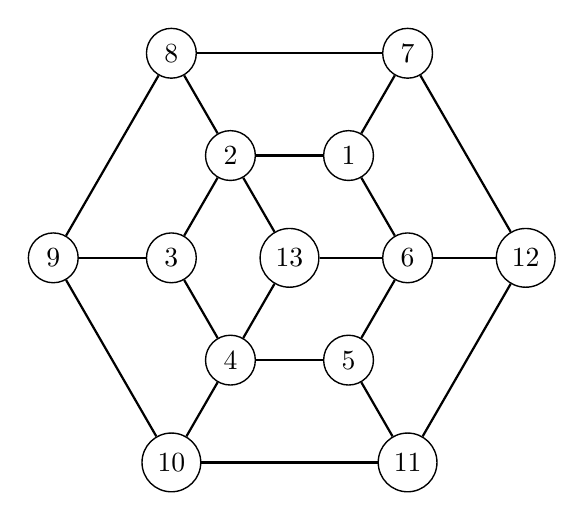
\begin{tikzpicture}
            \GraphInit[vstyle=Normal]
            \Vertex[a=0, d=0cm]{13}
            \foreach \t in {1,...,6}{%
                    \Vertex[a=0+60*\t,d=1.5cm]{\t}
                }
            \foreach \t in {7,...,12}{%
                    \Vertex[a=0+60*\t,d=3cm]{\t}
                }
            \Edges(1,2,3,4,5,6,1)
            \Edges(7,8,9,10,11,12,7)
            \Edges(1,7)
            \Edges(13,2,8)
            \Edges(3,9)
            \Edges(13,4,10)
            \Edges(5,11)
            \Edges(13,6,12)
        \end{tikzpicture}}
    \quad
    \subfigure[]{
        \begin{tikzpicture}
            \GraphInit[vstyle=Normal]
            \Vertex[a=0, d=0cm]{13}
            \foreach \t in {1,3,5}{%
                    \Vertex[a=0+60*\t,d=1.5cm]{\t}
                }
            \foreach \t in {8,10,12}{%
                    \Vertex[a=0+60*\t,d=3cm]{\t}
                }
        \end{tikzpicture}}
    \caption{第7题图(2)}
    \label{fig:8.5.2}
\end{figure}

\paragraph*{13} 考虑以人为顶点, 认识关系为边的无向图 $G$. 只需证明:
当 $n\ge3$时, $G$中存在哈密顿通路; 当 $n\ge4$时, $G$中存在哈密顿回路.

对于 $n=3$ 和 $n=4$ 的情形, 直接穷举可证. 以下考虑 $n\ge5$ 的情形.

任取 $G$ 中两个不相邻的顶点 $v_1, v_2$, 记剩余的顶点中, 与 $v_1$
相邻的顶点集为 $V_1$, 与 $v_2$ 相邻的顶点集为 $V_2$.
由条件知, $|V_1|+|V_2|\ge n-2\ge 3$, 根据鸽笼原理, $V_1$ 和 $V_2$
中至少有一个的顶点数不少于 $2$. 不妨设 $|V_1|\ge 2$.

那么可从 $V_1$ 中取两个顶点 $u_1, u_2$, 其中必有至少一个与 $v_2$ 相邻.
因此 $|V_1\cap V_2|\ge 1$, 故
$d(v_1)+d(v_2)=|V_1|+|V_2| = |V_1\cup V_2| + |V_1\cap V_2|\ge n-1$.
由定理 8.7 知, $G$ 中存在哈密顿通路.

设 $G$ 的一条哈密顿通路为 $v_1, v_2, \cdots, v_n$. 接下来参考定理 8.7 的证明,
可构造 $G$ 中的一条哈密顿回路.\QED

\newpage

\section*{习题九}

\paragraph*{2} 设 $T$ 中有 $x$ 个4度顶点, 那么由握手定理,
$9+3\times 3+4x=2(9+3+x-1)$, 解得 $x=2$. 即 $T$ 中有2个4度顶点.
度数列为 $4,4,3,3,3,1,1,1,1,1,1,1,1,1$.

以下用 \ding{174} 代表 3 度顶点, \ding{175} 代表 4 度顶点,
并省略所有叶子顶点.

如图\ref{fig:9.2.1}, 图\ref{fig:9.2.2}, 图\ref{fig:9.2.3} 所示,
共9种.

\begin{figure}[ht]
    \centering
    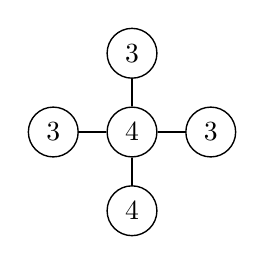
\begin{tikzpicture}
        \GraphInit[vstyle=Normal]
        \Vertex[L=3,x=0,y=0]{a}
        \Vertex[L=4,x=1,y=0]{b}
        \Vertex[L=3,x=2,y=0]{c}
        \Vertex[L=3,x=1,y=1]{d}
        \Vertex[L=4,x=1,y=-1]{e}
        \Edges(a,b,c)
        \Edges(d,b,e)
    \end{tikzpicture}
    \caption{第2题图: 直径为 5 的树}
    \label{fig:9.2.1}
\end{figure}

\begin{figure}[ht]
    \centering
    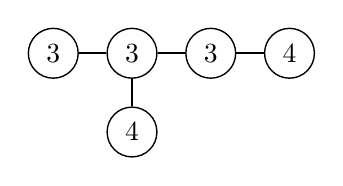
\begin{tikzpicture}
        \GraphInit[vstyle=Normal]
        \Vertex[L=3,x=0,y=0]{a}
        \Vertex[L=3,x=1,y=0]{b}
        \Vertex[L=3,x=2,y=0]{c}
        \Vertex[L=4,x=3,y=0]{d}
        \Vertex[L=4,x=1,y=-1]{e}
        \Edges(a,b,c,d)
        \Edges(b,e)
    \end{tikzpicture}
    \quad
    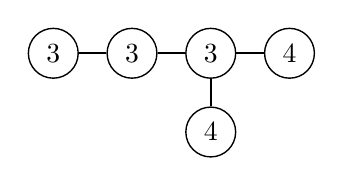
\begin{tikzpicture}
        \GraphInit[vstyle=Normal]
        \Vertex[L=3,x=0,y=0]{a}
        \Vertex[L=3,x=1,y=0]{b}
        \Vertex[L=3,x=2,y=0]{c}
        \Vertex[L=4,x=3,y=0]{d}
        \Vertex[L=4,x=2,y=-1]{e}
        \Edges(a,b,c,d)
        \Edges(c,e)
    \end{tikzpicture}
    \quad
    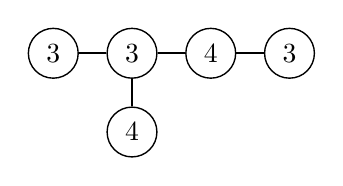
\begin{tikzpicture}
        \GraphInit[vstyle=Normal]
        \Vertex[L=3,x=0,y=0]{a}
        \Vertex[L=3,x=1,y=0]{b}
        \Vertex[L=4,x=2,y=0]{c}
        \Vertex[L=3,x=3,y=0]{d}
        \Vertex[L=4,x=1,y=-1]{e}
        \Edges(a,b,c,d)
        \Edges(b,e)
    \end{tikzpicture}
    \caption{第2题图: 直径为 6 的树}
    \label{fig:9.2.2}
\end{figure}

\begin{figure}[ht]
    \centering
    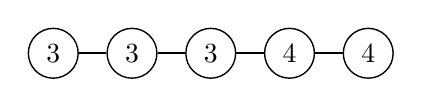
\begin{tikzpicture}
        \GraphInit[vstyle=Normal]
        \Vertex[L=3,x=0,y=0]{a}
        \Vertex[L=3,x=1,y=0]{b}
        \Vertex[L=3,x=2,y=0]{c}
        \Vertex[L=4,x=3,y=0]{d}
        \Vertex[L=4,x=4,y=0]{e}
        \Edges(a,b,c,d,e)
    \end{tikzpicture}
    \quad
    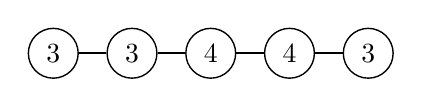
\begin{tikzpicture}
        \GraphInit[vstyle=Normal]
        \Vertex[L=3,x=0,y=0]{a}
        \Vertex[L=3,x=1,y=0]{b}
        \Vertex[L=4,x=2,y=0]{c}
        \Vertex[L=4,x=3,y=0]{d}
        \Vertex[L=3,x=4,y=0]{e}
        \Edges(a,b,c,d,e)
    \end{tikzpicture}
    \quad
    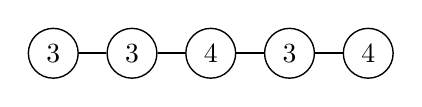
\begin{tikzpicture}
        \GraphInit[vstyle=Normal]
        \Vertex[L=3,x=0,y=0]{a}
        \Vertex[L=3,x=1,y=0]{b}
        \Vertex[L=4,x=2,y=0]{c}
        \Vertex[L=3,x=3,y=0]{d}
        \Vertex[L=4,x=4,y=0]{e}
        \Edges(a,b,c,d,e)
    \end{tikzpicture}
    \quad\\[2ex]
    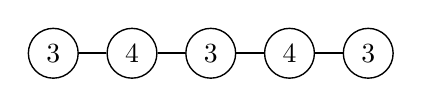
\begin{tikzpicture}
        \GraphInit[vstyle=Normal]
        \Vertex[L=3,x=0,y=0]{a}
        \Vertex[L=4,x=1,y=0]{b}
        \Vertex[L=3,x=2,y=0]{c}
        \Vertex[L=4,x=3,y=0]{d}
        \Vertex[L=3,x=4,y=0]{e}
        \Edges(a,b,c,d,e)
    \end{tikzpicture}
    \quad
    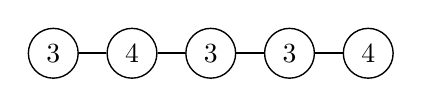
\begin{tikzpicture}
        \GraphInit[vstyle=Normal]
        \Vertex[L=3,x=0,y=0]{a}
        \Vertex[L=4,x=1,y=0]{b}
        \Vertex[L=3,x=2,y=0]{c}
        \Vertex[L=3,x=3,y=0]{d}
        \Vertex[L=4,x=4,y=0]{e}
        \Edges(a,b,c,d,e)
    \end{tikzpicture}
    \caption{第2题图: 直径为 7 的树}
    \label{fig:9.2.3}
\end{figure}

\paragraph*{6} 证明: 不妨设 $|E(G)|\ge |E(\overline{G})|$.

由 $|E(G)|+|E(\overline{G})| = n(n-1)/2$ 知, $|E(G)|\ge n(n-1)/4$.
假设 $G$ 中不含圈, 则 $G$ 中连通分支都是树, 设 $G$ 有 $k$ 个连通分支
$T_1, T_2, \ldots, T_k$, 则
\begin{align*}
    |E(G)| & = \sum_{i=1}^k |E(T_i)|    \\
           & = \sum_{i=1}^k |V(T_i)| -k \\
           & = n - k                    \\
           & \le n - 1                  \\
\end{align*}

即 $n-1 \le |E(G)| \le n(n-1)/4$, 解得 $1\le n\le 4$,
而$n\ge 5$, 矛盾. 故 $G$ 中必含圈. \QED

\paragraph*{11} 证明: 设$T$的树叶数目为 $k'$,
记 $T$ 的顶点个数为 $n$, 那么由握手定理,
\begin{align*}
    2(n-1) & \ge\Delta(T) + 2(n-k'-1) + k' \\
           & \ge k + 2(n-k'-1) + k'        \\
           & = 2(n-1) + k - k'             \\
\end{align*}
因此 $k'\ge k$, 即 $T$ 的树叶数目不少于 $k$. \QED

\newpage

\section*{习题十}

\paragraph*{2} 图的关联矩阵为
\begin{equation*}
    M(G) = \begin{pNiceMatrix}[first-row,first-col]
            & e_1 & e_2 & e_3 & e_4 & e_5 & e_6 \\
        v_1 & 1   & 0   & 0   & 1   & 0   & 0   \\
        v_2 & 0   & 1   & 1   & 1   & 0   & 0   \\
        v_3 & 0   & 0   & 1   & 0   & 1   & 0   \\
        v_4 & 1   & 1   & 0   & 0   & 1   & 1   \\
        v_5 & 0   & 0   & 0   & 0   & 0   & 1
    \end{pNiceMatrix}
\end{equation*}

以 $v_4$ 为参考点, 得基本关联矩阵

\begin{equation*}
    M_f(G) = \begin{pNiceMatrix}[first-row,first-col]
            & e_1 & e_2 & e_3 & e_4 & e_5 & e_6 \\
        v_1 & 1   & 0   & 0   & 1   & 0   & 0   \\
        v_2 & 0   & 1   & 1   & 1   & 0   & 0   \\
        v_3 & 0   & 0   & 1   & 0   & 1   & 0   \\
        v_5 & 0   & 0   & 0   & 0   & 0   & 1
    \end{pNiceMatrix}
\end{equation*}

注意到 $e_6$ 为桥, 故只需要考虑含 $e_6$ 的边集.

计算得
\begin{equation*}
    \begin{vNiceMatrix}[first-row,first-col]
            & e_1 & e_2 & e_3 & e_6 \\
        v_1 & 1   & 0   & 0   & 0   \\
        v_2 & 0   & 1   & 1   & 0   \\
        v_3 & 0   & 0   & 1   & 0   \\
        v_5 & 0   & 0   & 0   & 1
    \end{vNiceMatrix} = \begin{vNiceMatrix}
        1 & 1 \\
        0 & 1 \\
    \end{vNiceMatrix} = 1 \\
\end{equation*}

\begin{equation*}
    \begin{vNiceMatrix}[first-row,first-col]
            & e_1 & e_2 & e_4 & e_6 \\
        v_1 & 1   & 0   & 1   & 0   \\
        v_2 & 0   & 1   & 1   & 0   \\
        v_3 & 0   & 0   & 0   & 0   \\
        v_5 & 0   & 0   & 0   & 1
    \end{vNiceMatrix} = \begin{vNiceMatrix}
        1 & 0 & 1 \\
        0 & 1 & 1 \\
        0 & 0 & 0 \\
    \end{vNiceMatrix} = 0 \\
\end{equation*}

\begin{equation*}
    \begin{vNiceMatrix}[first-row,first-col]
            & e_1 & e_2 & e_5 & e_6 \\
        v_1 & 1   & 0   & 0   & 0   \\
        v_2 & 0   & 1   & 0   & 0   \\
        v_3 & 0   & 0   & 1   & 0   \\
        v_5 & 0   & 0   & 0   & 1
    \end{vNiceMatrix} = 1 \\
\end{equation*}

\begin{equation*}
    \begin{vNiceMatrix}[first-row,first-col]
            & e_1 & e_3 & e_4 & e_6 \\
        v_1 & 1   & 0   & 1   & 0   \\
        v_2 & 0   & 1   & 1   & 0   \\
        v_3 & 0   & 1   & 0   & 0   \\
        v_5 & 0   & 0   & 0   & 1
    \end{vNiceMatrix} = \begin{vNiceMatrix}
        1 & 0 & 1 \\
        0 & 1 & 1 \\
        0 & 1 & 0 \\
    \end{vNiceMatrix} = -1 \\
\end{equation*}

\begin{equation*}
    \begin{vNiceMatrix}[first-row,first-col]
            & e_1 & e_3 & e_5 & e_6 \\
        v_1 & 1   & 0   & 0   & 0   \\
        v_2 & 0   & 1   & 0   & 0   \\
        v_3 & 0   & 1   & 1   & 0   \\
        v_5 & 0   & 0   & 0   & 1
    \end{vNiceMatrix} = \begin{vNiceMatrix}
        1 & 0 & 0 \\
        0 & 1 & 0 \\
        0 & 1 & 1 \\
    \end{vNiceMatrix} = 1 \\
\end{equation*}

\begin{equation*}
    \begin{vNiceMatrix}[first-row,first-col]
            & e_1 & e_4 & e_5 & e_6 \\
        v_1 & 1   & 1   & 0   & 0   \\
        v_2 & 0   & 1   & 0   & 0   \\
        v_3 & 0   & 0   & 1   & 0   \\
        v_5 & 0   & 0   & 0   & 1
    \end{vNiceMatrix} = \begin{vNiceMatrix}
        1 & 1 & 0 \\
        0 & 1 & 0 \\
        0 & 0 & 1 \\
    \end{vNiceMatrix} = 1 \\
\end{equation*}


\begin{equation*}
    \begin{vNiceMatrix}[first-row,first-col]
            & e_2 & e_3 & e_4 & e_6 \\
        v_1 & 0   & 0   & 1   & 0   \\
        v_2 & 1   & 1   & 1   & 0   \\
        v_3 & 0   & 1   & 0   & 0   \\
        v_5 & 0   & 0   & 0   & 1
    \end{vNiceMatrix} = \begin{vNiceMatrix}
        0 & 0 & 1 \\
        1 & 1 & 1 \\
        0 & 1 & 0 \\
    \end{vNiceMatrix} = 1 \\
\end{equation*}

\begin{equation*}
    \begin{vNiceMatrix}[first-row,first-col]
            & e_2 & e_3 & e_5 & e_6 \\
        v_1 & 0   & 0   & 0   & 0   \\
        v_2 & 1   & 1   & 0   & 0   \\
        v_3 & 0   & 1   & 1   & 0   \\
        v_5 & 0   & 0   & 0   & 1
    \end{vNiceMatrix} = \begin{vNiceMatrix}
        0 & 0 & 0 \\
        1 & 1 & 0 \\
        0 & 1 & 1 \\
    \end{vNiceMatrix} = 0 \\
\end{equation*}

\begin{equation*}
    \begin{vNiceMatrix}[first-row,first-col]
            & e_2 & e_4 & e_5 & e_6 \\
        v_1 & 0   & 1   & 0   & 0   \\
        v_2 & 1   & 1   & 0   & 0   \\
        v_3 & 0   & 0   & 1   & 0   \\
        v_5 & 0   & 0   & 0   & 1
    \end{vNiceMatrix} = \begin{vNiceMatrix}
        0 & 1 & 0 \\
        1 & 1 & 0 \\
        0 & 0 & 1 \\
    \end{vNiceMatrix} = -1 \\
\end{equation*}

\begin{equation*}
    \begin{vNiceMatrix}[first-row,first-col]
            & e_3 & e_4 & e_5 & e_6 \\
        v_1 & 0   & 1   & 0   & 0   \\
        v_2 & 1   & 1   & 0   & 0   \\
        v_3 & 1   & 0   & 1   & 0   \\
        v_5 & 0   & 0   & 0   & 1
    \end{vNiceMatrix} = \begin{vNiceMatrix}
        0 & 1 & 0 \\
        1 & 1 & 0 \\
        1 & 0 & 1 \\
    \end{vNiceMatrix} = -1 \\
\end{equation*}

因此, 除 $e_1,e_2,e_4,e_6$ 和 $e_2,e_3,e_5,e_6$ 外,
以上列举的组合均为 $G$ 的生成树, 如图\ref{fig:10.2} 所示.

\begin{figure}[ht]
    \centering
    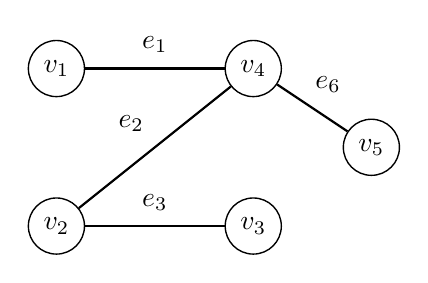
\begin{tikzpicture}
        \GraphInit[vstyle=Normal]
        \Vertex[L=$v_1$,x=0,y=2]{1}
        \Vertex[L=$v_2$,x=0,y=0]{2}
        \Vertex[L=$v_3$,x=2.5,y=0]{3}
        \Vertex[L=$v_4$,x=2.5,y=2]{4}
        \Vertex[L=$v_5$,x=4,y=1]{5}
        \Edge[label=$e_1$, labelstyle={shift={( 0.0, 0.3)}}](1)(4)
        \Edge[label=$e_2$, labelstyle={shift={(-0.3, 0.3)}}](2)(4)
        \Edge[label=$e_3$, labelstyle={shift={( 0.0, 0.3)}}](2)(3)
        % \Edge[label=$e_4$, labelstyle={shift={(-0.3, 0.0)}}](1)(2)
        % \Edge[label=$e_5$, labelstyle={shift={( 0.3, 0.0)}}](3)(4)
        \Edge[label=$e_6$, labelstyle={shift={( 0.2, 0.3)}}](4)(5)
    \end{tikzpicture}
    \quad
    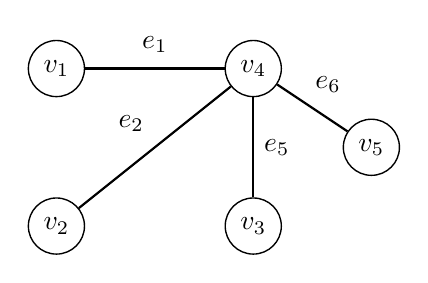
\begin{tikzpicture}
        \GraphInit[vstyle=Normal]
        \Vertex[L=$v_1$,x=0,y=2]{1}
        \Vertex[L=$v_2$,x=0,y=0]{2}
        \Vertex[L=$v_3$,x=2.5,y=0]{3}
        \Vertex[L=$v_4$,x=2.5,y=2]{4}
        \Vertex[L=$v_5$,x=4,y=1]{5}
        \Edge[label=$e_1$, labelstyle={shift={( 0.0, 0.3)}}](1)(4)
        \Edge[label=$e_2$, labelstyle={shift={(-0.3, 0.3)}}](2)(4)
        % \Edge[label=$e_3$, labelstyle={shift={( 0.0, 0.3)}}](2)(3)
        % \Edge[label=$e_4$, labelstyle={shift={(-0.3, 0.0)}}](1)(2)
        \Edge[label=$e_5$, labelstyle={shift={( 0.3, 0.0)}}](3)(4)
        \Edge[label=$e_6$, labelstyle={shift={( 0.2, 0.3)}}](4)(5)
    \end{tikzpicture}
    \quad
    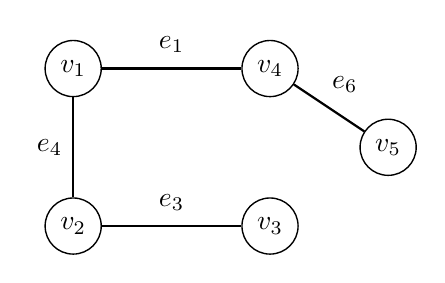
\begin{tikzpicture}
        \GraphInit[vstyle=Normal]
        \Vertex[L=$v_1$,x=0,y=2]{1}
        \Vertex[L=$v_2$,x=0,y=0]{2}
        \Vertex[L=$v_3$,x=2.5,y=0]{3}
        \Vertex[L=$v_4$,x=2.5,y=2]{4}
        \Vertex[L=$v_5$,x=4,y=1]{5}
        \Edge[label=$e_1$, labelstyle={shift={( 0.0, 0.3)}}](1)(4)
        % \Edge[label=$e_2$, labelstyle={shift={(-0.3, 0.3)}}](2)(4)
        \Edge[label=$e_3$, labelstyle={shift={( 0.0, 0.3)}}](2)(3)
        \Edge[label=$e_4$, labelstyle={shift={(-0.3, 0.0)}}](1)(2)
        % \Edge[label=$e_5$, labelstyle={shift={( 0.3, 0.0)}}](3)(4)
        \Edge[label=$e_6$, labelstyle={shift={( 0.2, 0.3)}}](4)(5)
    \end{tikzpicture}
    \quad\\[4ex]
    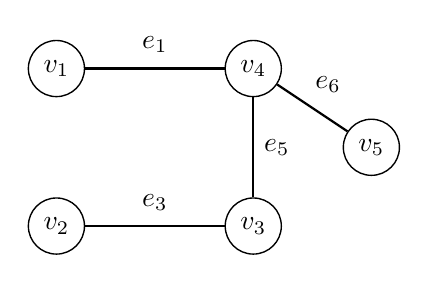
\begin{tikzpicture}
        \GraphInit[vstyle=Normal]
        \Vertex[L=$v_1$,x=0,y=2]{1}
        \Vertex[L=$v_2$,x=0,y=0]{2}
        \Vertex[L=$v_3$,x=2.5,y=0]{3}
        \Vertex[L=$v_4$,x=2.5,y=2]{4}
        \Vertex[L=$v_5$,x=4,y=1]{5}
        \Edge[label=$e_1$, labelstyle={shift={( 0.0, 0.3)}}](1)(4)
        % \Edge[label=$e_2$, labelstyle={shift={(-0.3, 0.3)}}](2)(4)
        \Edge[label=$e_3$, labelstyle={shift={( 0.0, 0.3)}}](2)(3)
        % \Edge[label=$e_4$, labelstyle={shift={(-0.3, 0.0)}}](1)(2)
        \Edge[label=$e_5$, labelstyle={shift={( 0.3, 0.0)}}](3)(4)
        \Edge[label=$e_6$, labelstyle={shift={( 0.2, 0.3)}}](4)(5)
    \end{tikzpicture}
    \quad
    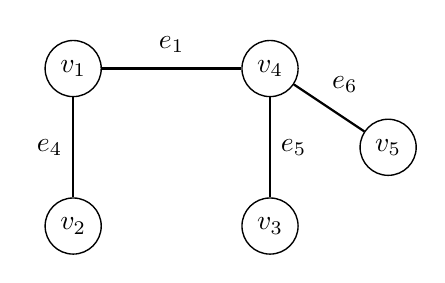
\begin{tikzpicture}
        \GraphInit[vstyle=Normal]
        \Vertex[L=$v_1$,x=0,y=2]{1}
        \Vertex[L=$v_2$,x=0,y=0]{2}
        \Vertex[L=$v_3$,x=2.5,y=0]{3}
        \Vertex[L=$v_4$,x=2.5,y=2]{4}
        \Vertex[L=$v_5$,x=4,y=1]{5}
        \Edge[label=$e_1$, labelstyle={shift={( 0.0, 0.3)}}](1)(4)
        % \Edge[label=$e_2$, labelstyle={shift={(-0.3, 0.3)}}](2)(4)
        % \Edge[label=$e_3$, labelstyle={shift={( 0.0, 0.3)}}](2)(3)
        \Edge[label=$e_4$, labelstyle={shift={(-0.3, 0.0)}}](1)(2)
        \Edge[label=$e_5$, labelstyle={shift={( 0.3, 0.0)}}](3)(4)
        \Edge[label=$e_6$, labelstyle={shift={( 0.2, 0.3)}}](4)(5)
    \end{tikzpicture}
    \quad
    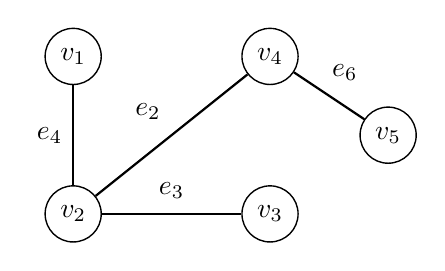
\begin{tikzpicture}
        \GraphInit[vstyle=Normal]
        \Vertex[L=$v_1$,x=0,y=2]{1}
        \Vertex[L=$v_2$,x=0,y=0]{2}
        \Vertex[L=$v_3$,x=2.5,y=0]{3}
        \Vertex[L=$v_4$,x=2.5,y=2]{4}
        \Vertex[L=$v_5$,x=4,y=1]{5}
        % \Edge[label=$e_1$, labelstyle={shift={( 0.0, 0.3)}}](1)(4)
        \Edge[label=$e_2$, labelstyle={shift={(-0.3, 0.3)}}](2)(4)
        \Edge[label=$e_3$, labelstyle={shift={( 0.0, 0.3)}}](2)(3)
        \Edge[label=$e_4$, labelstyle={shift={(-0.3, 0.0)}}](1)(2)
        % \Edge[label=$e_5$, labelstyle={shift={( 0.3, 0.0)}}](3)(4)
        \Edge[label=$e_6$, labelstyle={shift={( 0.2, 0.3)}}](4)(5)
    \end{tikzpicture}
    \quad\\[4ex]
    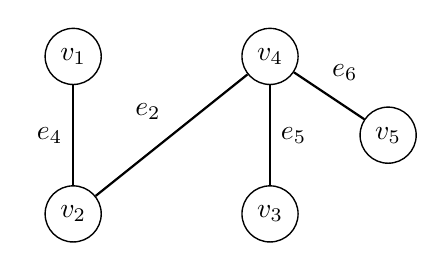
\begin{tikzpicture}
        \GraphInit[vstyle=Normal]
        \Vertex[L=$v_1$,x=0,y=2]{1}
        \Vertex[L=$v_2$,x=0,y=0]{2}
        \Vertex[L=$v_3$,x=2.5,y=0]{3}
        \Vertex[L=$v_4$,x=2.5,y=2]{4}
        \Vertex[L=$v_5$,x=4,y=1]{5}
        % \Edge[label=$e_1$, labelstyle={shift={( 0.0, 0.3)}}](1)(4)
        \Edge[label=$e_2$, labelstyle={shift={(-0.3, 0.3)}}](2)(4)
        % \Edge[label=$e_3$, labelstyle={shift={( 0.0, 0.3)}}](2)(3)
        \Edge[label=$e_4$, labelstyle={shift={(-0.3, 0.0)}}](1)(2)
        \Edge[label=$e_5$, labelstyle={shift={( 0.3, 0.0)}}](3)(4)
        \Edge[label=$e_6$, labelstyle={shift={( 0.2, 0.3)}}](4)(5)
    \end{tikzpicture}
    \quad
    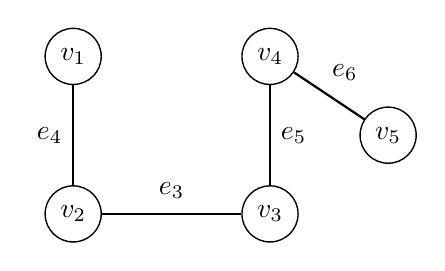
\begin{tikzpicture}
        \GraphInit[vstyle=Normal]
        \Vertex[L=$v_1$,x=0,y=2]{1}
        \Vertex[L=$v_2$,x=0,y=0]{2}
        \Vertex[L=$v_3$,x=2.5,y=0]{3}
        \Vertex[L=$v_4$,x=2.5,y=2]{4}
        \Vertex[L=$v_5$,x=4,y=1]{5}
        % \Edge[label=$e_1$, labelstyle={shift={( 0.0, 0.3)}}](1)(4)
        % \Edge[label=$e_2$, labelstyle={shift={(-0.3, 0.3)}}](2)(4)
        \Edge[label=$e_3$, labelstyle={shift={( 0.0, 0.3)}}](2)(3)
        \Edge[label=$e_4$, labelstyle={shift={(-0.3, 0.0)}}](1)(2)
        \Edge[label=$e_5$, labelstyle={shift={( 0.3, 0.0)}}](3)(4)
        \Edge[label=$e_6$, labelstyle={shift={( 0.2, 0.3)}}](4)(5)
    \end{tikzpicture}
    \caption{第2题图}
    \label{fig:10.2}
\end{figure}

\newpage

\paragraph*{4} $D$ 的邻接矩阵为
\begin{equation*}
    A = \begin{pNiceMatrix}[first-row,first-col]
            & v_1 & v_2 & v_3 & v_4 \\
        v_1 & 1   & 2   & 0   & 0   \\
        v_2 & 0   & 0   & 1   & 0   \\
        v_3 & 1   & 0   & 0   & 1   \\
        v_4 & 0   & 0   & 1   & 0   \\
    \end{pNiceMatrix}
\end{equation*}

计算得
\begin{equation*}
    A^2 = \begin{pNiceMatrix}[first-row,first-col]
            & v_1 & v_2 & v_3 & v_4 \\
        v_1 & 1   & 2   & 2   & 0   \\
        v_2 & 1   & 0   & 0   & 1   \\
        v_3 & 1   & 2   & 1   & 0   \\
        v_4 & 1   & 0   & 0   & 1   \\
    \end{pNiceMatrix},
    A^3 = \begin{pNiceMatrix}[first-row,first-col]
            & v_1 & v_2 & v_3 & v_4 \\
        v_1 & 3   & 2   & 2   & 2   \\
        v_2 & 1   & 2   & 1   & 0   \\
        v_3 & 2   & 2   & 2   & 1   \\
        v_4 & 1   & 2   & 1   & 0   \\
    \end{pNiceMatrix},
    A^4 = \begin{pNiceMatrix}[first-row,first-col]
            & v_1 & v_2 & v_3 & v_4 \\
        v_1 & 5   & 6   & 4   & 2   \\
        v_2 & 2   & 2   & 2   & 1   \\
        v_3 & 4   & 4   & 3   & 2   \\
        v_4 & 2   & 2   & 2   & 1   \\
    \end{pNiceMatrix};
\end{equation*}

\begin{equation*}
    B_2 = \begin{pNiceMatrix}[first-row,first-col]
            & v_1 & v_2 & v_3 & v_4 \\
        v_1 & 2   & 4   & 2   & 0   \\
        v_2 & 1   & 0   & 1   & 1   \\
        v_3 & 2   & 2   & 1   & 1   \\
        v_4 & 1   & 0   & 1   & 1   \\
    \end{pNiceMatrix},
    B_3 = \begin{pNiceMatrix}[first-row,first-col]
            & v_1 & v_2 & v_3 & v_4 \\
        v_1 & 5   & 6   & 4   & 2   \\
        v_2 & 2   & 2   & 2   & 1   \\
        v_3 & 4   & 4   & 3   & 2   \\
        v_4 & 2   & 2   & 2   & 1   \\
    \end{pNiceMatrix},
    B_4 = \begin{pNiceMatrix}[first-row,first-col]
            & v_1 & v_2 & v_3 & v_4 \\
        v_1 & 10  & 12  & 8   & 4   \\
        v_2 & 4   & 4   & 4   & 2   \\
        v_3 & 8   & 8   & 6   & 4   \\
        v_4 & 4   & 4   & 4   & 2   \\
    \end{pNiceMatrix};
\end{equation*}

\subparagraph*{(1)} 0,0,2,2;
\subparagraph*{(2)} 2;
\subparagraph*{(3)} 1,1,3,5;
\subparagraph*{(4)} 1;
\subparagraph*{(5)} 33;
\subparagraph*{(6)} 11;
\subparagraph*{(7)} 88,22;
\subparagraph*{(8)}
$\begin{pNiceMatrix}
        1 & 1 & 1 & 1 \\
        1 & 1 & 1 & 1 \\
        1 & 1 & 1 & 1 \\
        1 & 1 & 1 & 1 \\
    \end{pNiceMatrix}$.

\newpage

\section*{习题十一}

\paragraph*{6} 证明: 设面数为 $r$, 由欧拉公式, $n-m+r=7-15+r=2$,
解得 $r=10$. 记 $G$ 的面分别为 $R_1,R_2,\ldots,R_{10}$,
注意到 $\deg(R_i)\ge 3$, 有
\begin{equation*}
    30 = 2m = \sum_{i=1}^r\deg(R_i) \ge 3r = 30
\end{equation*}

因此不等号成立, 即 $\deg(R_i)=3, \forall i=1,2\ldots,r$.
故 $G$ 每个面次数均为3, $G$为极大平面图. \QED

\paragraph*{7} 证明: 不妨设 $|E(G)|\ge |E(\overline{G})|$.

由 $|E(G)|+|E(\overline{G})| = n(n-1)/2$ 知, $|E(G)|\ge n(n-1)/4$.
假设 $G$ 为平面图, 那么有 $|E(G)|\le 3n-6$,
故 $3n-6\ge n(n-1)/4$, 解得 $3\le n\le 10$.
而 $n\ge 11$, 矛盾, 因此 $G$ 不是平面图. \QED

\paragraph*{12} 证明: 由 $G$ 为极大平面图, 故 $G$ 中各面次数均为 3,
因此 $G^*$ 每个顶点的度数均为 3, 故 $G^*$ 为3-正则图.

又极大平面图一定为简单图, 故 $G$ 中无环, 因此$G^*$无桥, 因此$G^*$为2-边联通图.\QED

\paragraph*{16} 证明: 由握手定理,
\begin{equation*}
    3n = 2m = \sum_{i=3}^{\infty} i r_i
\end{equation*}

由欧拉定理,
\begin{align*}
    2 = n-m+r & = n-m + \sum_{i=3}^{\infty} r_i                                  \\
              & = -\frac{1}{6}\sum_{i=3}^{\infty} i r_i+ \sum_{i=3}^{\infty} r_i \\
              & =\frac{1}{6}\sum_{i=3}^{\infty} (6-i)r_i
\end{align*}

即
\begin{equation*}
    12 = \sum_{i=3}^{\infty} (6-i)r_i = 3r_3+2r_4+r_5 - r_7 - 2r_8 - 3r_9 - \cdots
\end{equation*}

\paragraph*{17} 证明: 记$G$的边数为 $m$, 由 $G$ 是外平面图,
$m\le 2n-3$, 故 $\overline{G}$ 的边数 $m'$ 满足
\begin{equation*}
    m' = \frac{n(n-1)}{2} - m \ge \frac{n(n-1)}{2} - 2n + 3
\end{equation*}

假设 $\overline{G}$ 也是平面图, 那么
\begin{equation*}
    \frac{n(n-1)}{2} - 2n + 3 \ge m' \ge 2n-3
\end{equation*}

解得 $2\le n \le 7$, 又 $n\ge 7$, 故 $n=7$, 因此 $10\le m,m'\le 11$.

不妨设 $m=11, m'=10$, 此时 $G$ 为极大外平面图, 至少有2个顶点度数为2.

注意到 $\overline{G}$ 为外平面图, 存在哈密顿回路,
即 $\overline{G}$ 中每个顶点的度数至少为2, 故
$G$ 中每个顶点的度数至多为4, 因此 $G$ 的度数列为 $4,4,3,3,3,2,2$ 或
$4,4,4,3,2,2,2$.

此时画图可知(见图\ref{fig:11.16.1}及图\ref{fig:11.16.2}),
$G$ 与 $\overline{G}$ 均无法同时是外平面图. \QED

\begin{figure}[ht]
    \centering
    \subfigure[$G$]{
        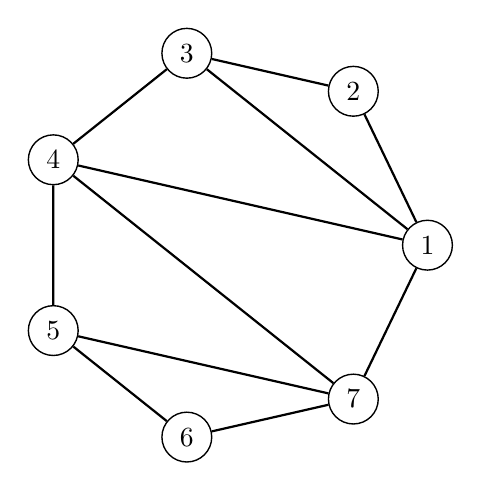
\begin{tikzpicture}
            \GraphInit[vstyle=Normal]
            \Vertices[unit=2.5]{circle}{1,2,3,4,5,6,7}
            \Edges(1,2,3,4,5,6,7,1)
            \Edges(1,3)
            \Edges(1,4)
            \Edges(4,7)
            \Edges(5,7)
        \end{tikzpicture}}
    \quad
    \subfigure[$\overline{G}$]{
        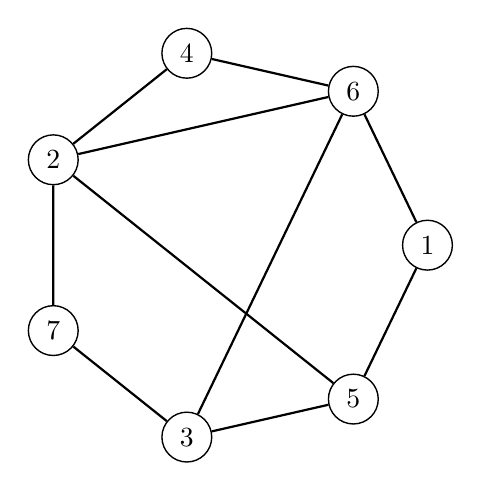
\begin{tikzpicture}
            \GraphInit[vstyle=Normal]
            % \Vertices[unit=2.5]{circle}{1,2,3,4,5,6,7}
            \Vertices[unit=2.5]{circle}{1,6,4,2,7,3,5}
            \Edges(1,6,4,2,7,3,5,1)
            \Edges(3,6,2,5)
        \end{tikzpicture}
    }
    \caption{第16题图(1)}
    \label{fig:11.16.1}
\end{figure}

\begin{figure}[ht]
    \centering
    \subfigure[$G$]{
        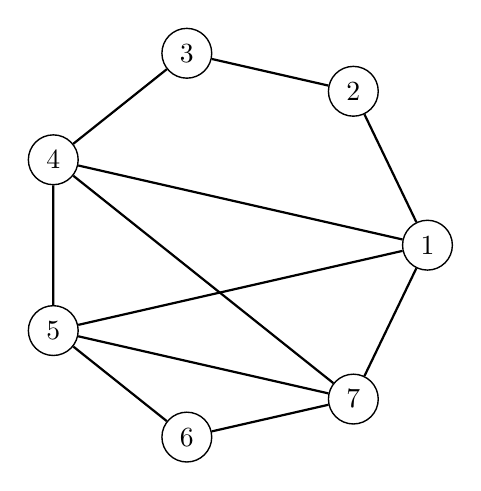
\begin{tikzpicture}
            \GraphInit[vstyle=Normal]
            \Vertices[unit=2.5]{circle}{1,2,3,4,5,6,7}
            \Edges(1,2,3,4,5,6,7,1)
            \Edges(1,5)
            \Edges(1,4)
            \Edges(4,7)
            \Edges(5,7)
        \end{tikzpicture}}
    \quad
    \subfigure[$\overline{G}$]{
        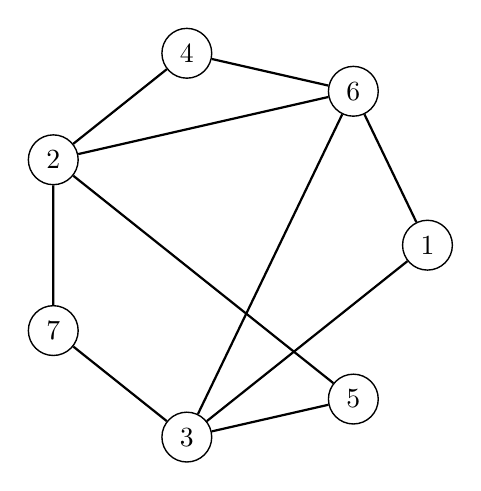
\begin{tikzpicture}
            \GraphInit[vstyle=Normal]
            % \Vertices[unit=2.5]{circle}{1,2,3,4,5,6,7}
            \Vertices[unit=2.5]{circle}{1,6,4,2,7,3,5}
            \Edges(1,6,4,2,7,3,1)
            \Edges(3,6,2,5,3)
        \end{tikzpicture}
    }
    \caption{第16题图(2)}
    \label{fig:11.16.2}
\end{figure}

\newpage

\paragraph*{18} 如图\ref{fig:11.18}, 一条哈密顿回路为
$v_1,v_2,v_3,v_4,v_5,v_{10},v_9,v_8,v_7,v_6,v_1$.
因此 $G$ 为哈密顿图.

\begin{figure}[ht]
    \centering
    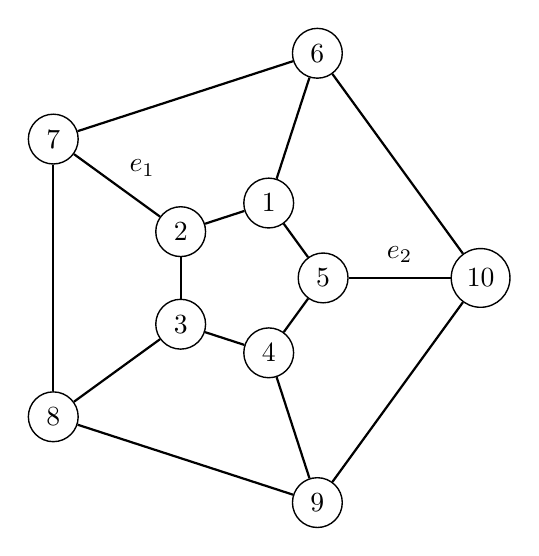
\begin{tikzpicture}
        \GraphInit[vstyle=Normal]
        \foreach \t in {1,...,5}{%
                \Vertex[a=0+72*\t,d=1cm]{\t}
            }
        \foreach \t in {6,...,10}{%
                \Vertex[a=0+72*\t,d=3cm]{\t}
            }        
        \Edges(1,2,3,4,5,1)
        \Edges(6,7,8,9,10,6)
        \Edges(1,6)
        \Edges[label=$e_1$, labelstyle={shift={( 0.32, 0.22)}}](2,7)
        \Edges(3,8)
        \Edges(4,9)
        \Edges[label=$e_2$, labelstyle={shift={( 0.0, 0.3)}}](5,10)
    \end{tikzpicture}
    \caption{第18题图}
    \label{fig:11.18}
\end{figure}

若存在经过 $e_1$ 和 $e_2$ 的哈密顿回路, 由定理11.23, 知
\begin{equation*}
    2(r_4'-r_4'') + 3(r_5'-r_5'') = 0
\end{equation*}

已知 $r_4'+r_4''=5$, $r_5'+r_5''=2$, 简单讨论可知
$r_5'=0, r_4'=4, r_5''=2, r_4''=1$ 或者
$r_5'=2, r_4'=1, r_5''=0, r_4''=4$. 这两种情况只是互换内外部的区别,
以下不妨设前者成立.

注意到 $e_1$ 是两个次数为4的面的边界, 
因此与其相邻的两个面至少有一个在哈密顿回路的外部,
同理 $e_2$ 也是如此. 而 $e_1$ 与 $e_2$ 没有公共的相邻面,
因此至少有2个面在哈密顿回路的外部, 与 $r_4''=1$ 矛盾. 
因此不存在经过 $e_1$ 和 $e_2$ 的哈密顿回路.

%第11章习题: 17,18


\end{document}

